\documentclass[a4paper]{article}

%% Language and font encodings
\usepackage[english]{babel}
\usepackage[utf8x]{inputenc}
\usepackage[T1]{fontenc}
%% Sets page size and margins
\usepackage[a4paper,top=3cm,bottom=2cm,left=3cm,right=3cm,marginparwidth=1.75cm]{geometry}

%% Useful packages
\usepackage{amsmath}
\usepackage{graphicx}
\usepackage[colorinlistoftodos]{todonotes}
\usepackage[colorlinks=true, allcolors=blue]{hyperref}
\usepackage{hyperref}
\usepackage{enumerate}

\title{Project IDS \\
Book Store using Google App Engine}
\author{LARREINEGABE Gerardo \\
RATNAPARKHI Gaurang \\
PERPETUA Patricio}
\date{9/04/2017}


\begin{document}
\maketitle


\section{Technologies Used}
\begin{itemize}
    
    \item Google App Engine (\url{https://cloud.google.com/appengine/})
    \item Google Cloud Postgresql (\url{https://cloud.google.com/sql/docs/postgres/})
    \item Google Cloud SDK (\url{https://cloud.google.com/sdk/})
    \item Docker (\url{https://www.docker.com/get-docker})
    \item Kubernetes (\url{https://kubernetes.io})
    \item Maven 
    \item Git
    \item Java Spring Boot
\end{itemize}

\section{Framework Used}
\begin{itemize}
    \item Yeoman (\url{http://yeoman.io/})
    \item Node.js (\url{https://nodejs.org/en/about/})
\end{itemize}
\subsection{Yeoman}
It is a generator ecosystem which it help us to proscribing best practices and tools to stay productive.
The workflow that it provides is a client-side stack, comprising tools and frameworks that can help quickly build web applications.
\subsection{Node}
Node.js is an event driven and therefore asynchronous I / O runtime library and environment that runs on the JavaScript interpreter created by Google V8. The truth is that it is very fashionable but not something new since there are libraries like Twisted that do exactly the same but if it is true that is the first based on JavaScript and has a great performance

\section{Logic}
The basic idea was to create a web application using JHipster and then deploy it on the Google Container engine using Kubernetes. The Google Cloud SQL was used as MySql backend.

\subsection{Why JHipster?}
JHipster uses the following Client Side (Front end) technologies
Yeoman, Webpack, Angular JS, Bootstrap.
Also it uses the following Server Side (Back end) technologies
Maven, Spring, Spring MVC REST, Spring data jpa.
It uses a ‘monolithic architecture’ which contains both front-end and back-end code.
It basically creates a decent architecture for the type of entities we want.

\subsection{Step-by-Step}
\subsection{Application}
\begin{itemize}
\item Create the environment on the local machine.
\item Create the structure of our application
\item Write logic for database entry and changes for UI.
\end{itemize}

\subsection{Docker and Kubernetes}

Following were the steps to deploy the web application \cite{docker}\cite{kubernetes}.

\begin{itemize}
    \item Create Google Cloud Project and set the project as default\\
    gcloud config set project bookstoreids
    \item Create a Google SQL Instance\\
    gcloud beta sql instances create bookstoresql --region=europe-west1 --tier=db-f1-micro\
 --authorized-networks=`curl -s ifconfig.co` --backup-start-time=01:00 --enable-bin-log \
 --activation-policy=ALWAYS --storage-type=HDD --storage-size=10GB
    \item Create a Container Cluster\\
    gcloud container clusters create bookstore-1 --zone=europe-west1-b --machine-type=g1-small --num-nodes=3
    \item Get the credentials for kubectl
    gcloud container clusters get-credentials bookstore-1
    \item Build and push a docker image \\ 
    docker image tag bookstore alarreine/bookstore:v1 \\
    It is better to add a version\\
    gcloud docker -- push bookstore alarreine/bookstore:v1
    \item Create Credentials to use Cloud SQL Proxy\\
    gcloud iam service-accounts create bookstore-app --display-name="Bookstore App"
    \item Get access to the service account
    gcloud projects add-iam-policy-binding bookstoreids \
 --member serviceAccount:service@created.com \
 --role roles/editor
 \item Create the key to use the proxy\\
 gcloud iam service-accounts keys create \
--iam-account service@created.com aplication-credentials.json
 \item Add this key to the cluster Kubernetes\\
 kubectl create secret generic cloudsql-oauth-credentials --from-file=credentials.json=aplication-credentials.json
 \item Add this credential to the pod file \cite{containersql}
\item Deploy the cluster \\
kubectl apply -f bookstore
\item Get the external IP \\
kubectl get services
 
\end{itemize}


\section{Architecture}
\subsection{Google Container}
The architecture of Google Container with Kubernetes Figure \ref{fig:googlecontainer}.


\subsection{Bookstore}
The architecture of Bookstore is 
Figure \ref{fig:bookstore}.

\begin{figure}
\centering
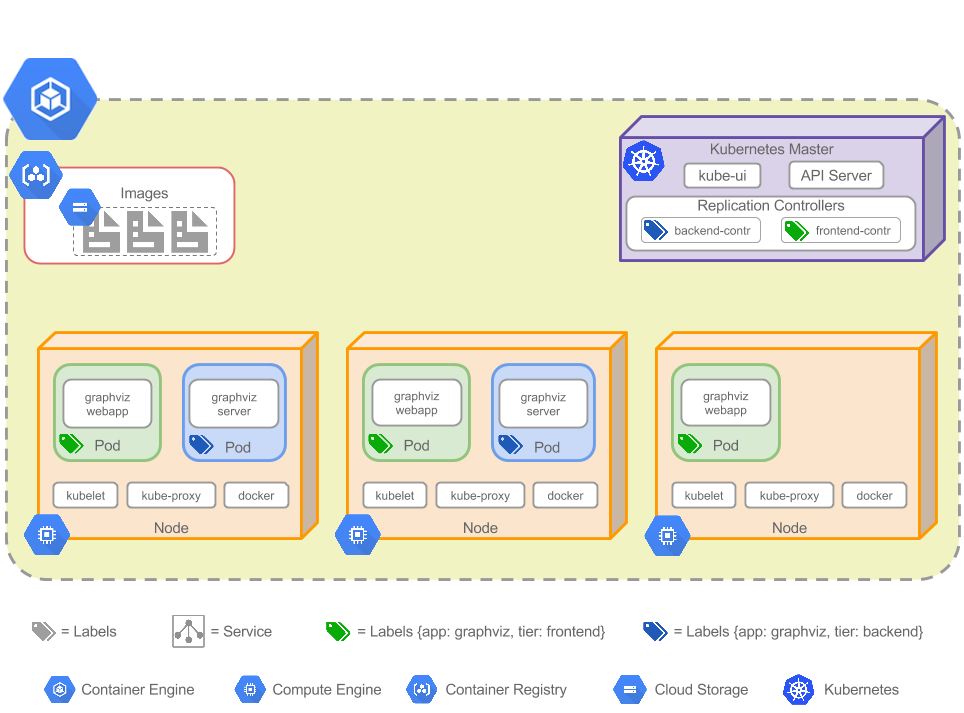
\includegraphics[width=0.5\textwidth]{grapheComputeEngine.png}
\caption{\label{fig:bookstore}Compute Engine.\cite{omerdawelbeit}}
\end{figure}

\begin{figure}
\centering
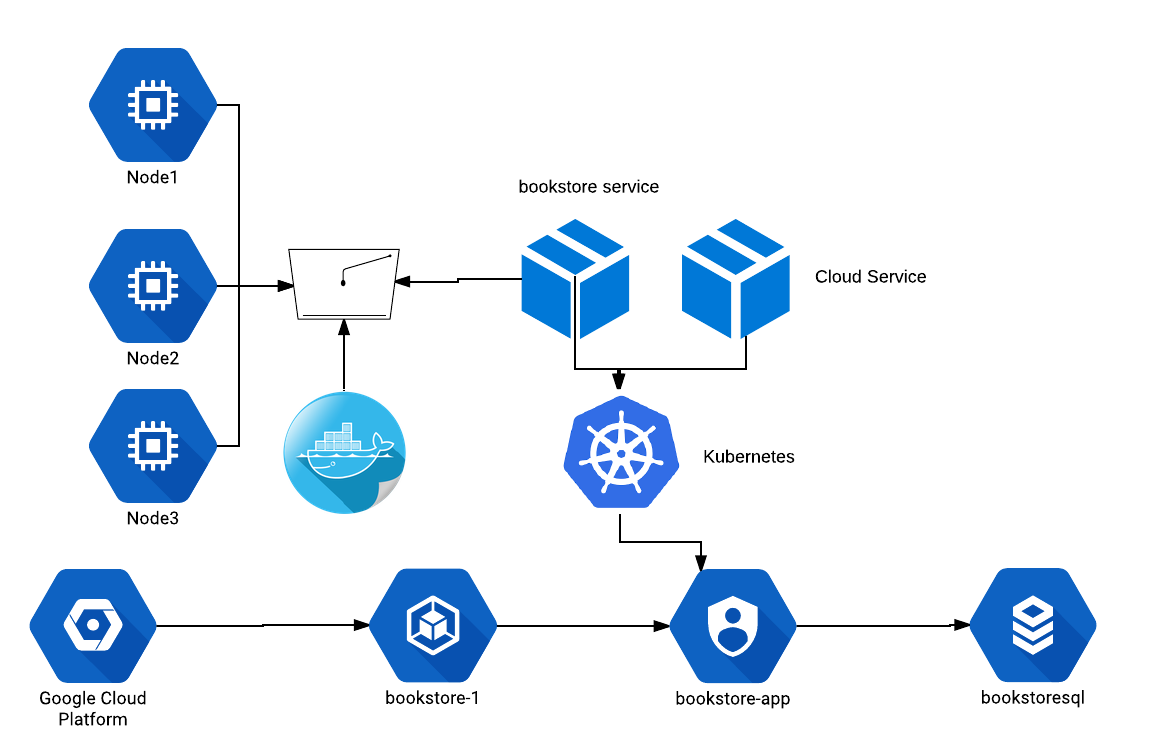
\includegraphics[width=0.5\textwidth]{bookstore.png}
\caption{\label{fig:bookstore}Architecture Bookstore.}
\end{figure}

\bibliographystyle{alpha}
\bibliography{sample}

\end{document}